% =====================================================================
%  THEORY v2 -- Coupled magnetic-mechanical oscillator
%  Lagrangian derivation (Rayleigh beam + dipole energy), Kelvin-Voigt
%  damping, normal modes, release problem; Extension: non-linear force.
%  Build:  tectonic -X compile theory_v2.tex      (figures: make_figs_v2.py)
% =====================================================================
\documentclass[11pt,a4paper]{article}
\usepackage[a4paper,margin=2.3cm]{geometry}
\usepackage[T1]{fontenc}\usepackage[utf8]{inputenc}\usepackage{lmodern}
\usepackage{amsmath,amssymb,bm}
\usepackage{booktabs,array}
\usepackage{enumitem}
\usepackage{xcolor}
\usepackage{graphicx}
\usepackage{tikz}
\usetikzlibrary{arrows.meta,calc,decorations.pathmorphing}
\usepackage{caption}
\captionsetup{font=small,labelfont=bf,width=0.92\textwidth}
\usepackage{tcolorbox}
\usepackage[hidelinks]{hyperref}

% ---- house style (same as the essay figures) ----
\colorlet{copper}{orange!80!black}
\colorlet{clampgray}{gray!60}
\colorlet{basegray}{gray!30}
\colorlet{magnetS}{red!70}
\colorlet{magnetN}{blue!70}
\newcommand{\magnetSN}[4]{%
  \fill[magnetS] (#1,#2) rectangle ({#1+#3/2},{#2+#4});
  \fill[magnetN] ({#1+#3/2},#2) rectangle ({#1+#3},{#2+#4});
  \node[white,font=\tiny] at ({#1+#3/4},{#2+#4/2}) {S};
  \node[white,font=\tiny] at ({#1+3*#3/4},{#2+#4/2}) {N};}
\newcommand{\magnetNS}[4]{%
  \fill[magnetN] (#1,#2) rectangle ({#1+#3/2},{#2+#4});
  \fill[magnetS] ({#1+#3/2},#2) rectangle ({#1+#3},{#2+#4});
  \node[white,font=\tiny] at ({#1+#3/4},{#2+#4/2}) {N};
  \node[white,font=\tiny] at ({#1+3*#3/4},{#2+#4/2}) {S};}
\newcommand{\muz}{\mu_0}
\newcommand{\mum}{\mu_{\mathrm m}}
\newcommand{\dd}{\mathrm{d}}
\newcommand{\un}[1]{\,\mathrm{#1}}
\newcommand{\Lag}{\mathcal L}
\newtcolorbox{keybox}{colback=blue!4,colframe=blue!50!black,boxrule=0.6pt,arc=2pt,left=4pt,right=4pt,top=3pt,bottom=3pt}
\newtcolorbox{notebox}{colback=gray!6,colframe=gray!55!black,boxrule=0.5pt,arc=2pt,left=4pt,right=4pt,top=3pt,bottom=3pt,fontupper=\small}

\setcounter{section}{4}

\begin{document}

\section{Theoretical model}\label{sec:theory}

The system is described by one Lagrangian: the kinetic and elastic energies of two vibrating cantilevers plus the interaction energy of two magnetic dipoles. Everything measured in this essay --- the two mode frequencies, their dependence on $d$, the peak heights, the beat minima, the decay --- follows from it. Sections \ref{sec:beam}--\ref{sec:release} develop the linear theory that the main analysis tests; Section~\ref{sec:nonlinear} (extension) keeps the full force law and predicts how the linear results fail as the magnets get close.

\subsection{Energy of one vibrating leaf spring}\label{sec:beam}

\begin{figure}[htbp]
\centering
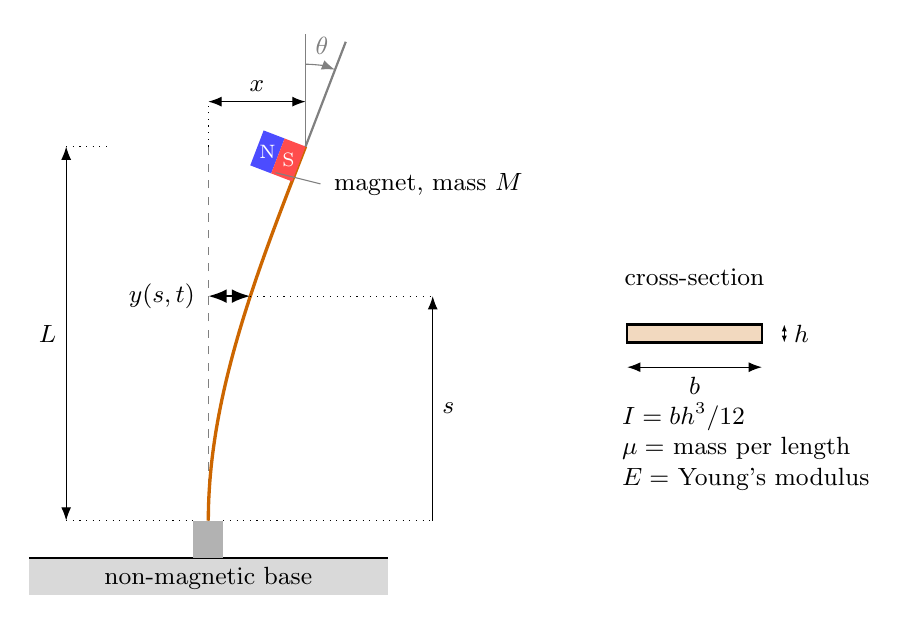
\begin{tikzpicture}[scale=0.95,>=Latex]
\fill[basegray] (-2.4,-0.5) rectangle (2.4,0);  \draw[thick] (-2.4,0)--(2.4,0);
\node[font=\small] at (0,-0.27) {non-magnetic base};
\fill[clampgray] (-0.2,0) rectangle (0.2,0.5);
\draw[dashed,gray] (0,0.5)--(0,5.5);
\draw[very thick,copper,domain=0:5,samples=50,variable=\s] plot ({1.3*\s*\s*(15-\s)/250},{0.5+\s});
\begin{scope}[shift={(1.3,5.5)},rotate=-21]
  \fill[magnetN] (-0.6,-0.5) rectangle (-0.3,0.0);
  \fill[magnetS] (-0.3,-0.5) rectangle (0.0,0.0);
  \node[white,font=\scriptsize] at (-0.45,-0.25){N}; \node[white,font=\scriptsize] at (-0.15,-0.25){S};
\end{scope}
\node[font=\small,anchor=west] at (1.55,5.0) {magnet, mass $M$};
\draw[gray,thin] (0.9,5.15)--(1.5,5.0);
\draw[<->] (0,6.1)--(1.3,6.1) node[midway,above,font=\small]{$x$};
\draw[dotted] (0,5.5)--(0,6.1);
\draw[<->] (-1.9,0.5)--(-1.9,5.5) node[midway,left,font=\small]{$L$};
\draw[dotted] (-1.9,0.5)--(-0.2,0.5); \draw[dotted] (-1.9,5.5)--(-1.35,5.5);
\draw[<->,thick] (0,3.5)--(0.56,3.5); \node[font=\small,anchor=east] at (-0.05,3.5){$y(s,t)$};
\draw[dotted] (0.56,3.5)--(3.0,3.5);
\draw[->] (3.0,0.5)--(3.0,3.5) node[midway,right,font=\small]{$s$};
\draw[dotted] (0.2,0.5)--(3.0,0.5);
% tip rotation theta = 3x/2L: tangent at the tip against the vertical
\draw[gray,thick] (1.3,5.5) -- ++(69:1.5); \draw[gray,thin] (1.3,5.5) -- (1.3,7.0);
\draw[gray,->] (1.3,6.6) arc (90:69:1.1); \node[gray,font=\small] at (1.52,6.85){$\theta$};
\begin{scope}[shift={(5.6,3.0)}]
\node[font=\small] at (0.9,0.75) {cross-section};
\draw[thick,fill=copper!25] (0,-0.12) rectangle (1.8,0.12);
\draw[<->] (0,-0.45)--(1.8,-0.45) node[midway,below,font=\small]{$b$};
\draw[{Latex[length=2.5pt]}-{Latex[length=2.5pt]}] (2.1,-0.12) -- (2.1,0.12) node[midway, right, font=\small]{$h$};
\node[font=\small,align=left,anchor=north west] at (-0.2,-0.8) {$I=bh^3/12$\\ $\mu=$ mass per length\\ $E=$ Young's modulus};
\end{scope}
\end{tikzpicture}
\caption{One leaf spring: free length $L$ above the clamp, lateral deflection $y(s,t)$, tip displacement $x(t)=y(L,t)$, tip rotation $\theta$, magnet of mass $M$ at the tip.}
\label{fig:cantilever}
\end{figure}

\paragraph{Separation of variables.} The strip is a thin elastic beam (Euler--Bernoulli: plane sections stay plane, deflections small). The lowest vibration mode of a cantilever with a heavy tip mass is, to very good accuracy, the \emph{static} deflection curve produced by a tip force \cite{gere,rao}:
\begin{equation}
y(s,t)=x(t)\,\varphi(s),\qquad \varphi(s)=\frac{3Ls^2-s^3}{2L^3},\qquad \varphi(0)=\varphi'(0)=0,\ \varphi(L)=1,\ \varphi''(L)=0.
\label{eq:shape}
\end{equation}
The shape satisfies the clamped conditions at $s=0$ and zero bending moment at the free tip. Only the tip coordinate $x(t)$ is then a dynamical variable --- the beam has been reduced to one degree of freedom (Rayleigh's method).

\paragraph{Kinetic and elastic energy.} Every element $\mu\,\dd s$ of the strip moves with velocity $\dot x\varphi(s)$; the magnet moves with $\dot x$. With bending energy $\tfrac12 EI\int (y'')^2\dd s$ (strain energy of a bent beam, \cite{gere}):
\begin{align}
T_{\rm beam}&=\tfrac12\mu\dot x^2\!\int_0^L\!\varphi^2\,\dd s=\tfrac12\Bigl(\tfrac{33}{140}\mu L\Bigr)\dot x^2,\qquad
T_{\rm magnet}=\tfrac12 M\dot x^2,\label{eq:T}\\
V_{\rm beam}&=\tfrac12 EI x^2\!\int_0^L\!(\varphi'')^2\,\dd s=\tfrac12\Bigl(\tfrac{3EI}{L^3}\Bigr)x^2\equiv\tfrac12 kx^2,\qquad k=\frac{Ebh^3}{4L^3}.\label{eq:V}
\end{align}
(The integrals: $\int_0^L\varphi^2\dd s=\tfrac{33}{140}L$ and $\int_0^L\varphi''^2\dd s=3/L^3$.) So one spring with its magnet is a harmonic oscillator with
\begin{equation}
m=M+\tfrac{33}{140}\mu L,\qquad k=\frac{Ebh^3}{4L^3},\qquad \omega_0^2=\frac km .
\label{eq:mk}
\end{equation}
How good is the one-mode reduction? Compared with the exact Euler--Bernoulli solution for a cantilever with a tip mass, \eqref{eq:mk} overestimates $\omega_0$ by $1.5\,\%$ for $M=0$ and by less than $0.2\,\%$ once $M>\tfrac12\mu L$, which is the case here. The next beam mode lies at $\gtrsim6\omega_0$ and is not excited by a slow tip release.

\begin{notebox}
\textbf{Tip rotation and gravity.} Two by-products of the shape function are used later. (i) The tip \emph{rotates} by $\theta=\varphi'(L)x=3x/2L$: the magnet is not translated but tilted, which changes the dipole interaction at second order (Section~\ref{sec:magnet}). (ii) The strip and magnet also \emph{descend} as they bend, by $\tfrac12\int\varphi'^2\dd s\,x^2=\tfrac35x^2/L$ at the tip; gravity therefore softens the stiffness by $\Delta k=-(1.2M+0.375\mu L)g/L$ --- an inverted-pendulum effect that, at $\omega_0\approx41\un{s^{-1}}$ and $L\approx0.2\un{m}$, amounts to a few per cent of $k$. It is included automatically when $k$ is measured with the strip vertical, and is noted when $k$ is compared with $Ebh^3/4L^3$.
\end{notebox}

\subsection{Energy of two interacting magnets}\label{sec:magnet}

Each magnet is a dipole of moment $\mum$; magnet 2 sits in the field of magnet 1. With the moments $\bm\mu_1,\bm\mu_2$ and the separation vector $\bm r$ from 1 to 2, the general dipole--dipole energy is \cite{griffiths}
\begin{equation}
U=-\bm\mu_2\!\cdot\!\bm B_1=\frac{\muz}{4\pi r^3}\Bigl[\bm\mu_1\!\cdot\!\bm\mu_2-3(\bm\mu_1\!\cdot\!\hat{\bm r})(\bm\mu_2\!\cdot\!\hat{\bm r})\Bigr].
\label{eq:Ugen}
\end{equation}
In the apparatus both moments lie along the line joining the magnets, pointing \emph{towards} each other (like poles facing), and each is tilted by its tip angle $\theta_i=3x_i/2L$. Inserting $\bm\mu_1=\mum(\cos\theta_1,\sin\theta_1)$, $\bm\mu_2=-\mum(\cos\theta_2,\sin\theta_2)$ and $\bm r=(d+x_2-x_1,\,0)$ (the tips stay at the same height to first order):
\begin{equation}
U(x_1,x_2)=\frac{\muz\mum^2}{4\pi (d+x_2-x_1)^3}\bigl[2\cos\theta_1\cos\theta_2-\sin\theta_1\sin\theta_2\bigr].
\label{eq:Utilt}
\end{equation}
The bracket equals $2$ for parallel, untilted moments (the form used in most treatments); the cosines and sines carry the tilt. The repulsive force between untilted coaxial magnets is
\begin{equation}
F(r)=-\frac{\partial}{\partial r}\Bigl(\frac{\muz\mum^2}{2\pi r^3}\Bigr)=\frac{3\muz\mum^2}{2\pi r^4}.
\label{eq:F}
\end{equation}

\begin{figure}[htbp]
\centering
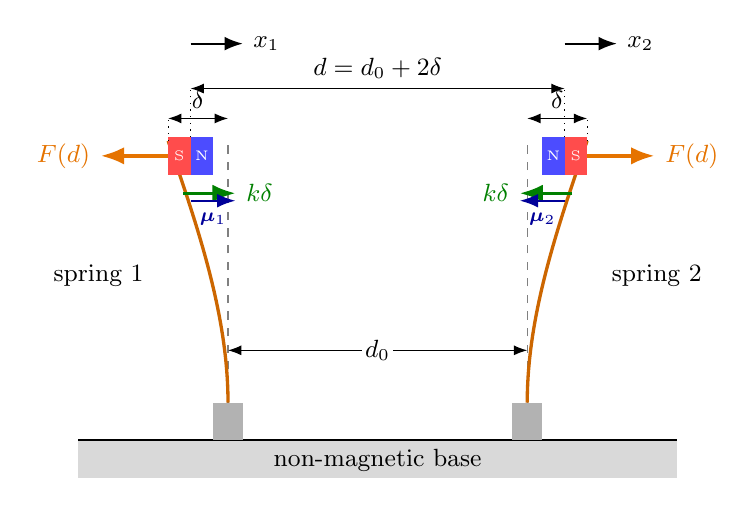
\begin{tikzpicture}[scale=0.95,>=Latex]
\fill[basegray] (-4.0,-0.5) rectangle (4.0,0); \draw[thick] (-4.0,0)--(4.0,0);
\node[font=\small] at (0,-0.27) {non-magnetic base};
\foreach \sx in {-1,1}{
  \fill[clampgray] ({\sx*2.0-0.2},0) rectangle ({\sx*2.0+0.2},0.5);
  \draw[dashed,gray] ({\sx*2.0},0.5)--({\sx*2.0},4.0);
  \draw[very thick,copper,domain=0:3.5,samples=40,variable=\s]
        plot ({\sx*2.0+\sx*0.8*\s*\s*(10.5-\s)/85.75},{0.5+\s});
}
\magnetSN{-2.8}{3.55}{0.6}{0.5}
\magnetNS{2.2}{3.55}{0.6}{0.5}
\node[font=\small,anchor=east] at (-3.0,2.2) {spring 1}; \node[font=\small,anchor=west] at (3.0,2.2) {spring 2};
\draw[<->] (-2.0,1.2)--(2.0,1.2) node[midway,fill=white,inner sep=1pt,font=\small]{$d_0$};
\draw[<->] (-2.5,4.7)--(2.5,4.7) node[midway,above,font=\small]{$d=d_0+2\delta$};
\draw[dotted] (-2.5,4.05)--(-2.5,4.7); \draw[dotted] (2.5,4.05)--(2.5,4.7);
\draw[<->] (2.0,4.3)--(2.8,4.3) node[midway,above,font=\small]{$\delta$};
\draw[<->] (-2.8,4.3)--(-2.0,4.3) node[midway,above,font=\small]{$\delta$};
\draw[dotted] (2.8,4.0)--(2.8,4.3); \draw[dotted] (-2.8,4.0)--(-2.8,4.3);
\draw[->,very thick,orange!90!black] (2.8,3.8)--(3.7,3.8) node[right,font=\small]{$F(d)$};
\draw[->,very thick,orange!90!black] (-2.8,3.8)--(-3.7,3.8) node[left,font=\small]{$F(d)$};
\draw[->,very thick,green!50!black] (2.6,3.3)--(1.9,3.3) node[left,font=\small]{$k\delta$};
\draw[->,very thick,green!50!black] (-2.6,3.3)--(-1.9,3.3) node[right,font=\small]{$k\delta$};
\draw[->,thick] (-2.5,5.3)--(-1.8,5.3) node[right,font=\small]{$x_1$};
\draw[->,thick] (2.5,5.3)--(3.2,5.3) node[right,font=\small]{$x_2$};
% moments
\draw[->,thick,blue!60!black] (-2.5,3.2)--(-1.9,3.2); \node[blue!60!black,font=\scriptsize] at (-2.2,2.95){$\bm\mu_1$};
\draw[->,thick,blue!60!black] (2.5,3.2)--(1.9,3.2); \node[blue!60!black,font=\scriptsize] at (2.2,2.95){$\bm\mu_2$};
\end{tikzpicture}
\caption{Equilibrium and coordinates. Mounting the second magnet bends each spring outwards by $\delta$ ($k\delta=F(d)$); the centre-to-centre separation $d$ is defined and measured in this state. $x_1,x_2$ are measured from the equilibrium positions, both positive to the right; the moments $\bm\mu_1,\bm\mu_2$ point towards each other.}
\label{fig:equilibrium}
\end{figure}

\subsection{Lagrangian and equations of motion}\label{sec:lagrangian}

With $x_1,x_2$ measured from the \emph{unstressed} positions of the springs for the moment,
\begin{equation}
\Lag=T-V=\tfrac12 m(\dot x_1^2+\dot x_2^2)-\tfrac12 k(x_1^2+x_2^2)-U(x_1,x_2).
\label{eq:L}
\end{equation}
Lagrange's equations $\frac{\dd}{\dd t}\frac{\partial\Lag}{\partial\dot x_i}=\frac{\partial\Lag}{\partial x_i}$ give
\begin{equation}
m\ddot x_1=-kx_1-\frac{\partial U}{\partial x_1},\qquad m\ddot x_2=-kx_2-\frac{\partial U}{\partial x_2}.
\label{eq:eom_full}
\end{equation}
For untilted moments $-\partial U/\partial x_1=-F(r)$ and $-\partial U/\partial x_2=+F(r)$ with $r$ the current separation: the repulsion pushes magnet 1 left and magnet 2 right. Equations~\eqref{eq:eom_full} are exact within the dipole and one-mode approximations; they are non-linear because $F\propto r^{-4}$, and Section~\ref{sec:nonlinear} solves them as they stand. The main analysis uses their linearisation.

\paragraph{Equilibrium.} At rest $kx_1=-F(d)$, $kx_2=+F(d)$: each spring is bent outwards by $\delta=F(d)/k$ and the magnets settle at $d=d_0+2\delta$ (Figure~\ref{fig:equilibrium}). From now on $x_1,x_2$ denote displacements from \emph{these} positions; the constant forces cancel.

\paragraph{Small oscillations.} Expanding $U$ to second order in $x_1,x_2$ (and in the tilt angles) about equilibrium,
\begin{equation}
\begin{aligned}
U&\simeq U_0+F(d)(x_1-x_2)+\tfrac12\gamma(x_2-x_1)^2-\frac{\gamma d^2}{128L^2}\bigl[9\,(x_1+x_2)^2+3\,(x_2-x_1)^2\bigr]+\dots,\\
\gamma&\equiv-\frac{\dd F}{\dd r}\Big|_{d}=\frac{4F(d)}{d}=\frac{6\muz\mum^2}{\pi d^5}.
\end{aligned}
\label{eq:Uquad}
\end{equation}
The first-order term is the equilibrium force already balanced by $k\delta$. The term $\tfrac12\gamma(x_2-x_1)^2$ is the energy of a spring of stiffness $\gamma$ --- the \emph{magnetic stiffness} --- joining the two magnets: repulsion that weakens with distance behaves, for small changes of separation, like a compressed spring. The last term is the tilt correction of \eqref{eq:Utilt}: it lowers $\omega_1^2$ and $\omega_2^2$ by the relative amounts $\frac{9}{32}\frac{\gamma}{k}(d/L)^2$ and $\frac{3}{32}g\,(d/L)^2$ ($g=\gamma/(k+2\gamma)$), i.e.\ by less than $10^{-3}$ for $d\le42\un{mm}$ and $L\ge150\un{mm}$ --- below the FFT resolution --- and is dropped (Section~\ref{sec:nonlinear} lists it among the neglected effects). The linear equations of motion are therefore
\begin{equation}
\boxed{\;m\ddot x_1=-kx_1+\gamma(x_2-x_1),\qquad m\ddot x_2=-kx_2-\gamma(x_2-x_1)\;}
\label{eq:eom}
\end{equation}
--- two equal masses on equal springs $k$, coupled by a spring $\gamma$.

\subsection{Normal modes}\label{sec:modes}

The symmetry of \eqref{eq:eom} under $1\leftrightarrow2$ suggests the coordinates
\begin{equation}
\eta=x_1+x_2\ \ (\text{centre of mass}),\qquad \xi=x_2-x_1\ \ (\text{change of separation}).
\end{equation}
Adding and subtracting the two equations decouples them:
\begin{equation}
m\ddot\eta=-k\eta,\qquad m\ddot\xi=-(k+2\gamma)\xi
\quad\Longrightarrow\quad
\boxed{\;\omega_1^2=\frac km,\qquad \omega_2^2=\frac{k+2\gamma}{m}\;}
\label{eq:modes}
\end{equation}
In the \emph{in-phase} mode ($\xi=0$) the separation never changes, the magnetic force stays at its equilibrium value and each spring swings as if alone at $\omega_1$, whatever $d$ is. In the \emph{anti-phase} mode ($\eta=0$) a displacement $a$ of each magnet changes the separation by $2a$, adding a force $2\gamma a$ to $ka$: stiffness $k+2\gamma$. In the Lagrangian picture, $\Lag=\tfrac14m(\dot\eta^2+\dot\xi^2)-\tfrac14k\eta^2-\tfrac14(k+2\gamma)\xi^2$ is a sum of two independent oscillators.

\begin{figure}[htbp]
\centering
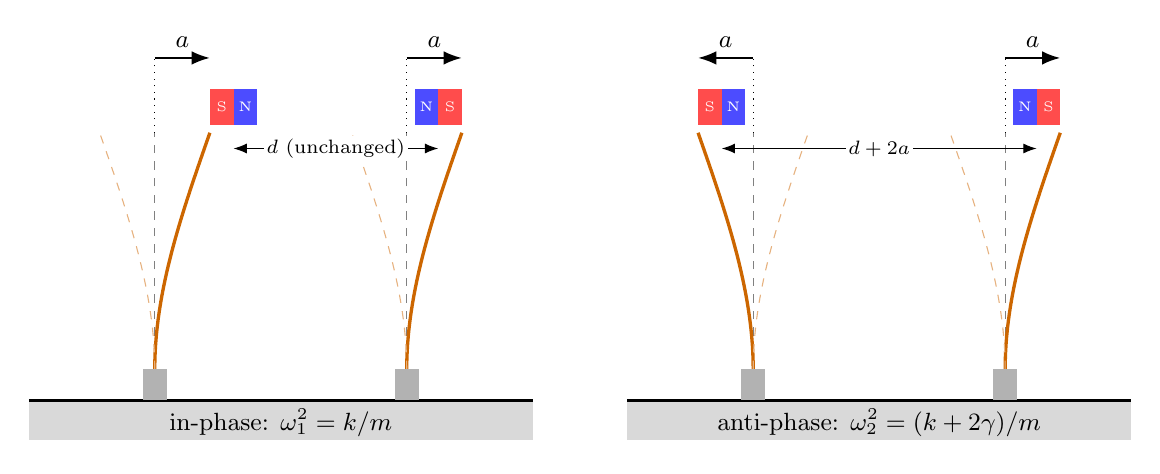
\begin{tikzpicture}[scale=1.0,>=Latex]
% ---- in-phase: both tips displaced to the right by a ----
\begin{scope}[shift={(0,0)}]
\fill[basegray] (-3.2,-0.5) rectangle (3.2,0); \draw[thick] (-3.2,0)--(3.2,0);
\foreach \sx in {-1,1}{
  \fill[clampgray] ({\sx*1.6-0.15},0) rectangle ({\sx*1.6+0.15},0.4);
  \draw[dashed,gray,thin] ({\sx*1.6},0.4)--({\sx*1.6},3.4);
  \draw[very thick,copper,domain=0:3,samples=30,variable=\s] plot ({\sx*1.6+0.7*\s*\s*(9-\s)/54},{0.4+\s});
  \draw[copper!50,dashed,domain=0:3,samples=30,variable=\s] plot ({\sx*1.6-0.7*\s*\s*(9-\s)/54},{0.4+\s});
}
% tips at x = -0.9 and +2.3; magnets on the inner faces
\magnetSN{-0.9}{3.5}{0.6}{0.45}
\magnetNS{1.7}{3.5}{0.6}{0.45}
\draw[->,thick] (-1.6,4.35)--(-0.9,4.35) node[midway,above,font=\small]{$a$};
\draw[->,thick] (1.6,4.35)--(2.3,4.35) node[midway,above,font=\small]{$a$};
\draw[dotted] (-1.6,3.4)--(-1.6,4.35); \draw[dotted] (1.6,3.4)--(1.6,4.35);
\draw[<->,thin] (-0.6,3.2)--(2.0,3.2) node[midway,fill=white,inner sep=1pt,font=\scriptsize]{$d$ (unchanged)};
\node[font=\small] at (0,-0.28) {in-phase: $\omega_1^2=k/m$};
\end{scope}
% ---- anti-phase: tips displaced outwards by a ----
\begin{scope}[shift={(7.6,0)}]
\fill[basegray] (-3.2,-0.5) rectangle (3.2,0); \draw[thick] (-3.2,0)--(3.2,0);
\foreach \sx in {-1,1}{
  \fill[clampgray] ({\sx*1.6-0.15},0) rectangle ({\sx*1.6+0.15},0.4);
  \draw[dashed,gray,thin] ({\sx*1.6},0.4)--({\sx*1.6},3.4);
  \draw[very thick,copper,domain=0:3,samples=30,variable=\s] plot ({\sx*1.6+\sx*0.7*\s*\s*(9-\s)/54},{0.4+\s});
  \draw[copper!50,dashed,domain=0:3,samples=30,variable=\s] plot ({\sx*1.6-\sx*0.7*\s*\s*(9-\s)/54},{0.4+\s});
}
% tips at x = -2.3 and +2.3
\magnetSN{-2.3}{3.5}{0.6}{0.45}
\magnetNS{1.7}{3.5}{0.6}{0.45}
\draw[->,thick] (-1.6,4.35)--(-2.3,4.35) node[midway,above,font=\small]{$a$};
\draw[->,thick] (1.6,4.35)--(2.3,4.35) node[midway,above,font=\small]{$a$};
\draw[dotted] (-1.6,3.4)--(-1.6,4.35); \draw[dotted] (1.6,3.4)--(1.6,4.35);
\draw[<->,thin] (-2.0,3.2)--(2.0,3.2) node[midway,fill=white,inner sep=1pt,font=\scriptsize]{$d+2a$};
\node[font=\small] at (0,-0.28) {anti-phase: $\omega_2^2=(k+2\gamma)/m$};
\end{scope}
\end{tikzpicture}
\caption{The two normal modes (solid: one extreme of the swing; dashed: the other; magnets drawn at the solid extreme). Left: both magnets move together, the separation and hence the magnetic force never change. Right: they move oppositely; the separation changes by $2a$, so the coupling spring $\gamma$ adds a force $2\gamma a$ to $ka$ on each magnet.}
\label{fig:modes}
\end{figure}

\begin{keybox}
\textbf{The relation tested by the experiment.} Subtracting the two mode frequencies removes $k$ and $m$:
\begin{equation}
f_2^2-f_1^2=\frac{\gamma}{2\pi^2 m}=\frac{3\muz\mum^2}{\pi^3 m}\,d^{-5}\equiv C\,d^{-5},
\qquad \ln\!\bigl(f_2^2-f_1^2\bigr)=\ln C-5\ln d .
\label{eq:main}
\end{equation}
$f_1$ should be independent of $d$; $f_2^2-f_1^2$ against $d$ on log--log axes should be a straight line of gradient $-5$ (Figure~\ref{fig:prediction}). The intercept gives $C$ and hence $\mum$ if $m$ is known --- or, with $\mum$ from the data sheet, an absolute test. The size of the coupling is $2\gamma/k=(f_2/f_1)^2-1\approx0.36$ at the closest separation used ($24.5\un{mm}$): the magnetic ``spring'' is about a fifth as stiff as the copper one.
\end{keybox}

\begin{figure}[htbp]\centering
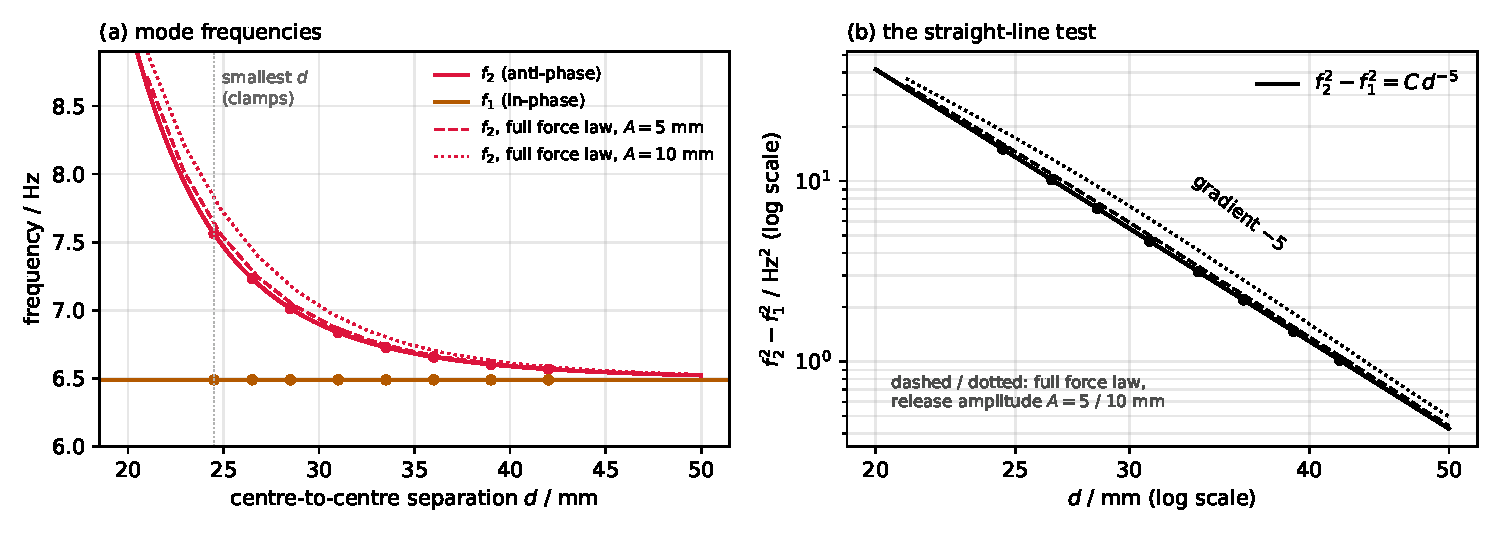
\includegraphics[width=\textwidth]{fig_prediction.pdf}
\caption{The prediction, drawn with the constants of the pilot run ($f_1=6.49\un{Hz}$, $C=1.33\times10^{-7}\un{m^5s^{-2}}$). Solid: linear model. (a) $f_1$ is flat; $f_2$ rises steeply below $30\un{mm}$. (b) $f_2^2-f_1^2$ on logarithmic axes: a line of gradient exactly $-5$. Dots: the separations used. Dashed and dotted: the same quantities from the full $r^{-4}$ force law (Section~\ref{sec:nonlinear}) for release amplitudes $A=5$ and $10\un{mm}$ --- the measured points are expected to lie slightly \emph{above} the line at the smallest $d$, by an amount that grows with $A^2$.}
\label{fig:prediction}
\end{figure}

\subsection{Damping: the Kelvin--Voigt beam}\label{sec:damping}

Copper is not perfectly elastic. The simplest model of internal friction in a solid is the Kelvin--Voigt model: the stress is $\sigma=E(\varepsilon+\tau_{\rm v}\dot\varepsilon)$, a spring and a dashpot in parallel, so that the bending moment acquires a term proportional to the \emph{rate of change of curvature} \cite{banks}:
\begin{equation}
\mathcal M=EI\Bigl(\frac{\partial^2y}{\partial s^2}+\tau_{\rm v}\frac{\partial^3 y}{\partial s^2\partial t}\Bigr)
\quad\Longrightarrow\quad
\mu\frac{\partial^2y}{\partial t^2}=-EI\frac{\partial^2}{\partial s^2}\Bigl(\frac{\partial^2y}{\partial s^2}+\tau_{\rm v}\frac{\partial^3y}{\partial s^2\partial t}\Bigr).
\label{eq:KV}
\end{equation}
With the one-mode ansatz $y=x(t)\varphi(s)$ the dissipative term produces, by exactly the same integral as $V_{\rm beam}$, a force $-k\tau_{\rm v}\dot x$ on the tip coordinate; air drag on the magnet adds a further term $-c_{\rm a}\dot x$. Both are linear in $\dot x$ and equal for the two identical springs, so in \eqref{eq:eom} $m\ddot x_i\to m\ddot x_i+c\,\dot x_i$ with $c=k\tau_{\rm v}+c_{\rm a}$, and the mode equations become
\begin{equation}
\ddot\eta+2\lambda\dot\eta+\omega_1^2\eta=0,\qquad \ddot\xi+2\lambda\dot\xi+\omega_2^2\xi=0,\qquad \lambda=\frac{c}{2m}=\frac1{\tau_d},
\end{equation}
with solutions $e^{-\lambda t}\cos(\omega_i't+\phi_i)$, $\omega_i'=\sqrt{\omega_i^2-\lambda^2}$. Three consequences are used in the analysis:
\begin{enumerate}[leftmargin=1.8em,itemsep=1pt]
\item \textbf{The frequencies are unaffected.} With $\tau_d\approx21\un{s}$ (pilot run) and $\omega\approx41\un{s^{-1}}$, $\lambda/\omega\approx10^{-3}$ and $\omega'-\omega\approx-\tfrac12\lambda^2/\omega\sim10^{-6}\omega$. Damping changes the peak \emph{width} (full width at half maximum of the power spectrum $1/\pi\tau_d\approx15\un{mHz}$), not the peak position.
\item \textbf{Both modes decay at the same rate}, because the same $c$ acts in both. The ratio of the two FFT peaks and the ratio of beat minima to maxima are then constant in time (Figure~\ref{fig:damping}a). A dissipation that depends on the \emph{relative} motion --- eddy currents induced in one magnet by the changing field of the other, or air squeezed in the gap --- would damp the anti-phase mode faster and make the beat minima rise with time (Figure~\ref{fig:damping}b). The envelope of the record therefore tests which damping mechanism operates.
\item \textbf{The KV coefficient is a material property}: $\lambda=k\tau_{\rm v}/2m+c_{\rm a}/2m$. Measuring $\tau_d$ for the ``Infinity'' recordings (one spring alone) and at each $d$ separates the two contributions: the KV part is the same for all $d$.
\end{enumerate}

\begin{figure}[htbp]\centering
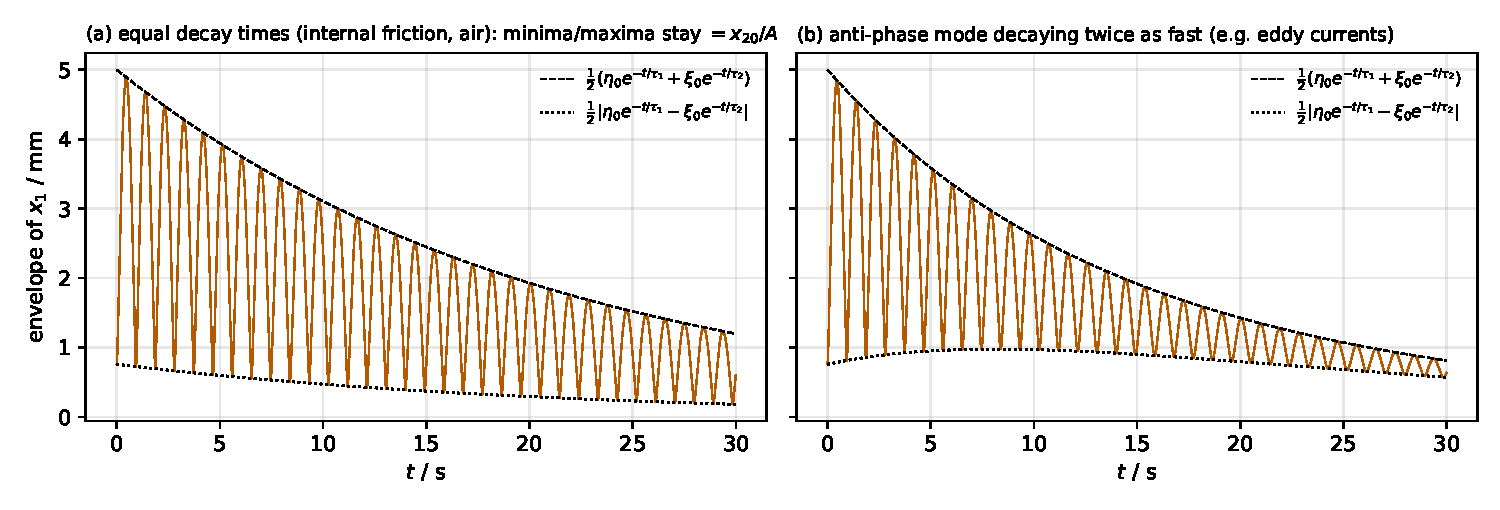
\includegraphics[width=\textwidth]{fig_damping.pdf}
\caption{The envelope of the released spring as a test of the damping model ($d=24.5\un{mm}$, $A=5\un{mm}$). (a) Equal decay of both modes (Kelvin--Voigt internal friction, air drag on each magnet): the ratio of beat minima to maxima stays fixed at $x_{20}/A$. (b) If the anti-phase mode decayed twice as fast, the minima would rise while the maxima fall.}
\label{fig:damping}
\end{figure}

\subsection{The release experiment: what the spectrum should show}\label{sec:release}

In the experiment spring 1 is pulled outwards by $A$, held until spring 2 is at rest, and released. While spring 1 is held at $x_1=-A$ (positive $x$ to the right), spring 2 feels a reduced repulsion and settles a distance $x_{20}=A\gamma/(k+\gamma)$ towards it, at $x_2=-x_{20}$ (from $kx_2=\gamma(x_1-x_2)$, the static form of \eqref{eq:eom}). Both start from rest, so the mode amplitudes are $\eta_0=-(A+x_{20})$ and $\xi_0=A-x_{20}$, and
\begin{equation}
x_1(t)=\tfrac12\bigl(\eta_0\cos\omega_1t-\xi_0\cos\omega_2t\bigr)e^{-\lambda t},\qquad
x_2(t)=\tfrac12\bigl(\eta_0\cos\omega_1t+\xi_0\cos\omega_2t\bigr)e^{-\lambda t}.
\label{eq:release}
\end{equation}
Each record contains both frequencies; the FFT of \emph{either} spring shows two peaks at $f_1$ and $f_2$ whose heights are in the ratio
\begin{equation}
\frac{\xi_0}{|\eta_0|}=\frac{A-x_{20}}{A+x_{20}}=\frac{k}{k+2\gamma}=\Bigl(\frac{f_1}{f_2}\Bigr)^{2}.
\label{eq:ratio}
\end{equation}
This is a prediction with no free parameter: at $d=24.5\un{mm}$ the anti-phase peak should be $0.74$ of the in-phase peak, for both springs. The positions of the peaks do not depend on how the motion was started; the heights do, and \eqref{eq:ratio} is what a hold-and-release start gives. The sum of two cosines is a fast oscillation at $f_{\rm avg}=\tfrac12(f_1+f_2)$ whose amplitude swells and shrinks with period
\begin{equation}
T_{\rm beat}=\frac1{f_2-f_1},\qquad\text{minima } \tfrac12|\eta_0|-\tfrac12\xi_0=x_{20},\quad\text{maxima } A,
\end{equation}
so the depth of the beat minima measures $x_{20}$ and hence $\gamma/k$ a third way (Figure~\ref{fig:release}). The energy travels back and forth: spring 2 is loudest when spring 1 is quietest, a quarter of a beat later.

\begin{figure}[htbp]\centering

\includegraphics[width=\textwidth]{fig_release.pdf}
\caption{Linear model with Kelvin--Voigt damping, $d=24.5\un{mm}$, $A=5\un{mm}$, $\tau_d=21\un{s}$. (a) Both springs: fast oscillation at $f_{\rm avg}$, envelope with period $T_{\rm beat}=1/(f_2-f_1)=0.93\un{s}$, minima at $x_{20}=0.76\un{mm}$; the envelopes of the two springs are a quarter-beat apart. (b) The spectra of the 45 s records: two peaks, the same positions for both springs, height ratio $(f_1/f_2)^2$.}
\label{fig:release}
\end{figure}

\subsection*{Summary of the linear model}
\begin{center}\small
\begin{tabular}{@{}p{6.6cm}lp{6.2cm}@{}}
\toprule
prediction & equation & how it is tested\\
\midrule
$f_1$ independent of $d$ & \eqref{eq:modes} & $f_1(d)$ flat; equals the single-spring frequency\\
$f_2^2-f_1^2=Cd^{-5}$ & \eqref{eq:main} & log--log gradient $-5$ (main graph)\\
peak-height ratio $(f_1/f_2)^2$, same for both springs & \eqref{eq:ratio} & FFT peak heights\\
beat minima $=x_{20}=A\gamma/(k+\gamma)$, period $1/(f_2-f_1)$ & \eqref{eq:release} & envelope of $x_1(t)$\\
equal decay of both modes & \S\ref{sec:damping} & min/max ratio constant in time\\
absolute value $C=3\muz\mum^2/\pi^3m$ & \eqref{eq:main} & $C$ from intercept vs data-sheet $\mum$, measured $m$\\
\bottomrule
\end{tabular}
\end{center}

% ======================================================================
\section{Extension: the non-linear force law}\label{sec:nonlinear}

The linearisation replaced $F(d+\xi)$ by its tangent. The true force $F\propto r^{-4}$ is convex: pushing the magnets together by $\xi$ raises the repulsion more than pulling them apart by $\xi$ lowers it. Keeping the full law in the mode equations shows what the linear model misses and when.

\paragraph{Exact mode equations.} Adding and subtracting \eqref{eq:eom_full} (untilted dipoles) gives, without approximation,
\begin{equation}
m\ddot\eta=-k\eta,\qquad m\ddot\xi=-k\xi+2\bigl[F(d+\xi)-F(d)\bigr].
\label{eq:exact}
\end{equation}
(Each magnet feels $\mp[F(d+\xi)-F(d)]$, the change of the repulsion from its equilibrium value; the difference of the two equations doubles it.) The centre-of-mass motion is \emph{exactly} harmonic at $\omega_1$: the magnetic force is internal and cancels from $\eta$ whatever its form. All non-linearity lives in the relative coordinate; for $\xi>0$ (magnets further apart) the bracket is negative, so the extra force is restoring, and the linear limit $-2\gamma\xi$ is recovered from $F'(d)=-\gamma$. Expanding $F(d+\xi)=F(d)(1+\xi/d)^{-4}$,
\begin{equation}
(1+u)^{-4}=1-4u+10u^2-20u^3+\dots,\qquad
\ddot\xi+\omega_2^2\,\xi=\omega_2^2\,g\Bigl[\,5\frac{\xi^2}{d}-10\frac{\xi^3}{d^2}+\dots\Bigr],\qquad g\equiv\frac{\gamma}{k+2\gamma},
\label{eq:xi_nl}
\end{equation}
where $\gamma=4F(d)/d$ was used. The parameter $g$ measures how much of the anti-phase stiffness is magnetic ($g=0.13$ at $24.5\un{mm}$, $0.05$ at $31\un{mm}$, $0.01$ at $42\un{mm}$), and the expansion parameter is $\xi/d$.

\paragraph{Perturbation solution.} Writing $\xi=a\cos\omega t+\dots$ and collecting terms (Lindstedt--Poincar\'e, to second order in $a/d$) gives
\begin{align}
\xi(t)&=\underbrace{\frac{5g}{2}\frac{a^2}{d}}_{\text{mean shift}}+a\cos\omega t-\underbrace{\frac{5g}{6}\frac{a^2}{d}\cos2\omega t}_{\text{2nd harmonic}}+\underbrace{\Bigl(\frac{5g}{16}+\frac{25g^2}{48}\Bigr)\frac{a^3}{d^2}\cos3\omega t}_{\text{3rd harmonic}}+\dots\label{eq:harmonics}\\[2pt]
\frac{\omega-\omega_2}{\omega_2}&=\Bigl(\frac ad\Bigr)^{2}\Bigl[\frac{15g}{4}-\frac{125g^2}{12}\Bigr]>0 .\label{eq:shift}
\end{align}
Three testable statements follow (all checked against a direct numerical integration of \eqref{eq:exact}, Figure~\ref{fig:nonlinear}):
\begin{enumerate}[leftmargin=1.8em,itemsep=2pt]
\item \textbf{$f_2$ depends on amplitude; $f_1$ never does.} The anti-phase frequency \emph{rises} with the square of the separation swing --- the convex force is stiffer on average than its tangent. For the hold-and-release start $a\approx\xi_0=A-x_{20}$; with $A=5\un{mm}$ the shift is $+0.9\,\%$ at $24.5\un{mm}$, $+0.4\,\%$ at $31\un{mm}$ and below $0.1\,\%$ beyond $36\un{mm}$; with $A=10\un{mm}$ it is four times larger. This is why the release amplitude is a controlled variable, why the measured log--log gradient is expected to bend \emph{above} $-5$ at the smallest $d$, and why an amplitude series at fixed $d$ is a direct test of \eqref{eq:shift}. In a damped record the amplitude decays during the measurement, so the FFT peak sits at a time-averaged shift, about $0.15$--$0.2$ of the initial-amplitude value for $\tau_d=21\un{s}$ and $T=45\un{s}$ (numerical result); the two-tone fit over the first few beats sees the full shift.
\item \textbf{Harmonics.} The relative motion contains $2f_2$ and $3f_2$ with relative amplitudes $\frac{5g}{6}\frac{\xi_0}{d}\approx2\,\%$ and $\approx0.15\,\%$ at $24.5\un{mm}$, $A=5\un{mm}$, and a mean outward shift $\frac{5g}{2}\xi_0^2/d\approx0.2\un{mm}$ (the magnets spend more time far apart than close). Since $x_{1,2}=\tfrac12(\eta\mp\xi)$, each spring's spectrum shows the harmonics of $f_2$ but not of $f_1$; combination tones $f_1\pm f_2$, $2f_1$ appear only through the (tiny) tilt coupling of \eqref{eq:Uquad}. A $2\,\%$ line is visible in a 45 s Hann spectrum with a $10^{3}$ dynamic range --- an optional check.
\item \textbf{Internal resonance.} If $\omega_2=2\omega_1$ the second harmonic of the anti-phase motion is resonant with the in-phase mode and energy can pass between modes even at small amplitude --- the ``critical value'' seen by other groups. Here $\omega_2^2/\omega_1^2=1+2\gamma/k=4$ requires $2\gamma/k=3$, i.e.\ $d^*=(C/3f_1^2)^{1/5}\approx16\un{mm}$: below the smallest separation the clamps allow ($24.5\un{mm}$, where $2\gamma/k=0.36$) and below the range in which the magnets can be treated as dipoles at all. The condition is therefore not met in this experiment, which is a strength: the two modes stay independent and the linear model remains applicable down to $24.5\un{mm}$, with the small amplitude corrections above.
\end{enumerate}

\begin{figure}[htbp]\centering
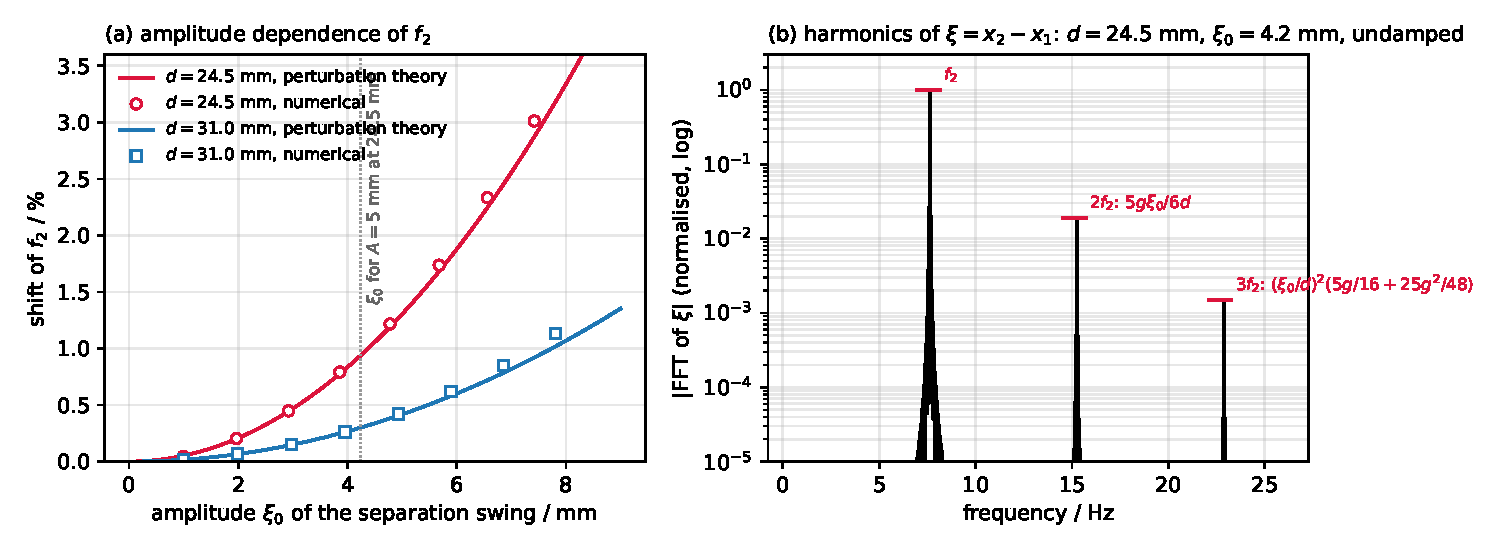
\includegraphics[width=\textwidth]{fig_nonlinear.pdf}
\caption{Non-linear predictions checked numerically. (a) Shift of $f_2$ against the amplitude of the separation swing at two separations: lines, equation~\eqref{eq:shift}; symbols, direct integration of \eqref{eq:exact}. The dotted line marks $\xi_0$ for the standard $A=5\un{mm}$ release at $24.5\un{mm}$. (b) Spectrum of $\xi(t)$ from the integration at $24.5\un{mm}$ (log scale): the harmonics at $2f_2$ and $3f_2$ have the relative sizes predicted by \eqref{eq:harmonics} (red bars).}
\label{fig:nonlinear}
\end{figure}

\paragraph{Other neglected effects, in order of size.} (i) \emph{Finite magnet size}: a disc magnet is a dipole only for $d\gg D$; the next multipole term changes $F$ by $O(D^2/d^2)$ and steepens the effective exponent at small $d$ --- fitted in the evaluation with the magnets modelled as two charged discs. (ii) \emph{Detuning}: if $k_1\ne k_2$ the modes mix, $(f_2^2-f_1^2)^2=(f_b^2-f_a^2)^2+(Cd^{-5})^2$, and the peak ratios of the two springs differ; measured by the ``Infinity'' recordings. (iii) \emph{Tip tilt}: relative corrections $\lesssim10^{-3}$ to both mode frequencies, equation~\eqref{eq:Uquad}. (iv) \emph{Gravity}: a few per cent of $k$, absorbed into the measured $k$. (v) \emph{Higher beam modes}: $\ge6\omega_1$, not excited by a slow release.

\begin{thebibliography}{9}\small
\bibitem{gere} J.~M. Gere and B.~J. Goodno, \emph{Mechanics of Materials}, 8th ed. (Cengage, 2012), ch.~9 (cantilever deflection) and ch.~5 (bending stress).
\bibitem{rao} S.~S. Rao, \emph{Mechanical Vibrations}, 6th ed. (Pearson, 2017), \S2.5 (Rayleigh's energy method) and \S8.5 (cantilever with tip mass).
\bibitem{griffiths} D.~J. Griffiths, \emph{Introduction to Electrodynamics}, 4th ed. (Cambridge, 2017), \S6.1 (force and energy of magnetic dipoles).
\bibitem{banks} H.~T. Banks and D.~J. Inman, ``On damping mechanisms in beams'', \emph{J. Appl. Mech.} \textbf{58}, 716--723 (1991) (Kelvin--Voigt and air damping of a cantilever).
\end{thebibliography}

\end{document}
